%%%%%%%%%%%%%%%%%%%%%%%%%%%%%%%%%%%%%%% PROBLEM FORMULATION OR STATEMENT %%%%%%%%%%%%%%%%%%%%%%%%%%%%%%


\chapter{Problem Statement}\label{chap:Problem_statement}

\section{Fusion Algorithm}\label{sec:2-bayes_fusion}
Fusing measurements from two heterogeneous sensors that have few cross-correlations can be challenging. 
To take inputs from two different sensors and give them weight, we use Bayes Fusion in this thesis.
Bayes fusion takes the noises of both sensors to determine their reliability at a given point of the measurement.
Thus giving us a reliable way to give scores of trust to each sensor.

The coordinates that undergo fusion from both radar and image sensors are the horizontal coordinates,
specifically the radar's azimuth and the image's "u" coordinate. 
This constraint arises from the fact that these are the only coordinates where both sensors provide measurements, 
as illustrated in Figure \ref{fig:trade_off_and_plane}\subref{subfig:cam_radar_sub}.
It's important to note that radar's elevation measurement resolution is limited and subject to noise. 
Additionally, the image sensor does not provide depth information.

If X is the real position of the object, 
then Bayes' theorem predicts that the probability of the fused position is shown in equation \ref{equ:bayes1} \cite{10.1007/978-981-16-2248-9_32}.

\begin{equation}\label{equ:bayes1}
    P_{prob}(\frac{P}{X})=
    \frac
    {e \frac{−(P−X)^T R^{−1}(P−X)}{2}}
    {2 \pi R^(0.5)}
\end{equation}

Applying Bayes' fusion, the value of the measured measurements is provided by equation \ref{equ:bayes2}.

\begingroup
\large
\begin{equation}\label{equ:bayes2}
\theta_{bayes}=\frac
{\frac{\theta_{radar}}{R_{radar}}+\frac{\theta_{cam}} {R_{cam}}}
{\frac{1}{R_{radar}}+\frac{1}{R_{cam}}}
\end{equation}
\endgroup

where
\begin{align*}
    \theta_{bayes} &= \text{fused position}\\
    \theta_{radar} &= \text{radar azimuth angle}\\
    \theta_{cam} &= \text{camera azimuth angle}\\
    R_{radar} &= \text{radar covariance}\\
    R_{cam} &= \text{camera covariance}
\end{align*}
\begin{equation}\label{equ:bayes4}
    \frac{1}{R}=\frac{1}{R_1}+\frac{1}{R_2}
\end{equation}
\begin{equation}\label{equ:2-radar_R}
    \mathbf{R}_{radar} = 
        \sigma_{radar_x}^2 
\end{equation}
\begin{equation}\label{equ:2-R_cam}
    \mathbf{R}_{cam} = 
        \sigma_{cam_u}^2
\end{equation}


\section{Motion Model}\label{sec:2-kalman_filter}
%To predict the movement model of our subjects, we use a Constant Acceleration model of Kalman filter.

\subsection{Predict}\label{sec:2-predict}
The state matrix used in this Kalman Filter \cite{kalman} is from the single sensor maneuvering tracking, with constant velocity.
It has four elements and is defined with position and velocity, which projects onto the x-axis and y-axis:

\begin{equation}\label{equ:state_eq}
    \mathbf{x} = 
        \begin{bmatrix} 
        p \\ 
        v \\

        \end{bmatrix} = 
        \begin{bmatrix} 
        p_x \\ 
        p_y \\ 
        v_x \\ 
        v_y \\
        \end{bmatrix}
\end{equation}
where
\begin{align*}
    p_x &=\text{position x}\\
    p_y &=\text{position y}\\
    v_x &=\text{velocity x}\\
    v_y &=\text{velocity y}\\
\end{align*}

\begin{equation}\label{equ:transition_matrix_H}
    \mathbf{F} = 
    \begin{bmatrix}
        1 & 0 & 1 & 0 \\
        0 & 1 & 0 & 1 \\
        0 & 0 & 0 & 0 \\
        0 & 0 & 0 & 0 \\
      \end{bmatrix}
\end{equation}

\begin{equation}\label{equ:predict_eq}
    \mathbf{x}_k=\mathbf{F}_k\mathbf{x}_{k-1}+\mathbf{w}
\end{equation}

Error covariance update
\begin{equation}\label{equ:error_covariance}
    \mathbf{P}_k=\mathbf{F}_k \mathbf{P}_{k-1} \mathbf{F}_k^T+\mathbf{Q}_k
\end{equation}

\newpage
\subsection{Update}\label{equ:2_update}
To fuse two sensors with different update rates, Kalman Filter is updated seperately (figure \ref{fig:sync_fig}).
Updates are based on the fps of each sensor.
\begin{figure}[hpbt]
    \centering
    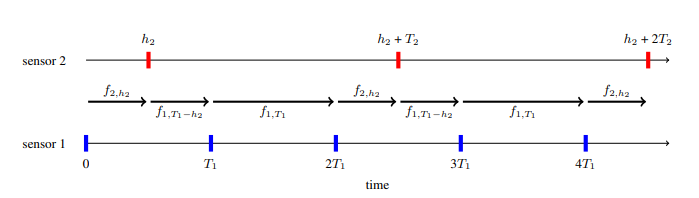
\includegraphics[width=\textwidth]{Figures/sync.png}%\textwidth
    \caption{Update timing \cite{7472511}}
    \label{fig:sync_fig}
\end{figure}


Both radar and camera undergo the same update procedure within the Kalman filter framework. 
Nevertheless, variations exist in their measurement data, 
leading to distinct measurement matrices and noise covariance. 
Radar measurements encompass two parameters: azimuth and range, 
both presented in polar coordinates. 
These radar coordinates are derived from the centroids of the k-d tree clusters.


\begin{equation}
    \mathbf{z}=
    \begin{bmatrix}
        \rho \\ 
        \theta_{bayes}\\
    \end{bmatrix}
\end{equation}


After the measurement matrix $\mathbf{z}_k$ is obtained, 
it is subtracted from the previously predicted values by the Kalman Filter. 
\begin{equation}
    \mathbf{y}_{k}=\mathbf{z}-\mathbf{H}_k \mathbf{x}_k
\end{equation}
Subsequently, the matrix $ \mathbf{G}_k $ is calculated to determine the trustworthiness of the current measurement, taking into account measurement noise. 
\begin{equation}
    \mathbf{G}_k = \frac{\mathbf{P}_k \mathbf{H}_k^T}{\mathbf{H}_k\mathbf{P}_k\mathbf{H}_k^T + \mathbf{R}_k}
\end{equation}
Finally, the current state estimation is updated based on this adjusted measurement.
\begin{equation}
    \mathbf{P}_k = (\mathbf{I} - \mathbf{G}_k\mathbf{H})\mathbf{P}_k
\end{equation}

\newpage

\subsection{Non-linearity}\label{equ:2_non_linear}
EKF
\begin{equation}
    h(\mathbf{x}_k)=
    \begin{bmatrix}
        \rho \\ 
        \theta_{bayes}\\
    \end{bmatrix}=
    \begin{bmatrix}
    \sqrt{p_x^2+p_y^2}\\
    \tan^{-1}(\frac{p_x}{p_y})
    \end{bmatrix}
    \end{equation}
    Transition matrix
    \begingroup
        \large
        \begin{equation}
            \mathbf{H}=
            \begin{bmatrix}
                \frac{\partial h(\mathbf{x}_k)}{\partial \mathbf{x}_k}
            \end{bmatrix}=
            \begin{bmatrix}
                \frac{\partial \rho}{\partial p_x} & \frac{\partial \rho}{\partial p_y}
                & \frac{\partial \rho}{\partial v_x}& \frac{\partial \rho}{\partial v_y} \\
        
                \frac{\partial \theta}{\partial p_x} & \frac{\partial \theta}{\partial p_y} 
                & \frac{\partial \theta}{\partial v_x}& \frac{\partial \theta}{\partial v_y} \\
            \end{bmatrix}
        \end{equation}
        
        \begin{equation}
            \mathbf{H}=
            \begin{bmatrix}
                \frac{p_x}{\sqrt{p_x^2+p_y^2}} & \frac{p_y}{\sqrt{p_x^2+p_y^2}} & 0 & 0 \\
                -\frac{p_y}{p_x^2+p_y^2} & \frac{p_x}{p_x^2+p_y^2} & 0 & 0 \\
            \end{bmatrix}
        \end{equation}
    \endgroup